% !TEX root =  ../pers_schedules.tex 
\section{Simulation Study}
\label{sec: simulation_study}
The application of personalized schedules for patients from PRIAS demonstrated that these schedules adapt according to the historical data of each patient. However we could not perform a full scale comparison between personalized and PRIAS schedule, because the true time of GR was not known for the PRIAS patients. To this end, we conducted a simulation study comparing personalized schedules with PRIAS and annual schedule, whose details are presented next.

\subsection{Simulation Setup}
\label{subsec : simulation_setup}
First we assume a population of patients enrolled in AS, with the same entrance criteria as that of PRIAS. The PSA and hazard of GR for patients from this population follow a joint model of the form postulated in Section \ref{subsec : jm_fit_prias}, with parameters equal to the posterior mean of parameters estimated from the joint model fitted to PRIAS dataset (Web Appendix C of the supplementary material). We further assume that there are three equal sized subgroups $G_1$, $G_2$ and $G_3$ of patients in the population, differing in the baseline hazard of GR. This was done because we wanted to test the performance of different schedules for a population with a mixture of patients, namely those with faster progressing PCa, as well as those with slowly progressing PCa. For the three subgroups we use a Weibull distributed baseline hazard with the following shape and scale parameters $(k, \lambda$): $(1.5, 4)$, $(3, 5)$ and $(4.5, 6)$ for $G_1, G_2$ and $G_3$, respectively. The effect of these parameters is that the mean GR time is lowest in $G_1$ (faster progressing PCa) and highest in $G_3$ (slowly progressing PCa).

From this population we have sampled 500 datasets with 1000 patients each. Patients are randomly assigned to a subgroup. Further, each dataset is split into a training (750 patients) and a test (250 patients) part. The $k$-th simulated training dataset $\mathcal{D}^k$ is given by $\mathcal{D}^k = \{l_{ki}, r_{ki}, \boldsymbol{y}_{ki}; i = 1, \ldots, 750\}$, where $\boldsymbol{y}_{ki}$ denote the PSA measurements for the $i$-th patient in $\mathcal{D}^k$. The frequency of PSA measurements is same as that in PRIAS. Other than simulating a true GR time $T^*_{ki}$, we also generate a random and non-informative censoring time $C_{ki}$. When $T^*_{ki} < C_{ki}$, then $l_{ki} = r_{ki} = T^*_{ki}$, otherwise $l_{ki} = C_{ki}$ and $r_{ki} = \infty$. For the test patients, censoring time is not generated.

We next fit a joint model of the specification given in (\ref{eq : long_model_prias}) and (\ref{eq : hazard_prias}) to each of the $\mathcal{D}^k, k=1, \ldots, 500$, and obtain a MCMC sample from the posterior distribution $p(\boldsymbol{\theta} \mid \mathcal{D}^k)$. We then obtain $g(T^*_{kl})$ for each of the $l$-th test patient of the $k$-th data set and conduct hypothetical biopsies for him. For every patient we conduct biopsies using the following six types of schedules (abbreviated names in parenthesis): personalized schedules based on expected time of GR (Exp. GR time) and median time of GR (Med. GR time), personalized schedules based on dynamic risk of GR (Dyn. risk GR), a hybrid approach between median time of GR and dynamic risk of GR (Hybrid), PRIAS schedule and annual schedule. The biopsies are conducted iteratively in accordance with the algorithm in Figure \ref{fig : sched_algorithm}. 

To compare the aforementioned schedules we require estimates of the various criteria based on offset and number of biopsies conducted to detect GR (Section \ref{sec : choosing_schedule}). To this end, we compute pooled estimates of each of the $E(N^S_j)$, $\mbox{var}(N^S_j)$, $E(O^S_j)$ and $\mbox{var}(O^S_j)$, as below:
\begin{align*}
\widehat{E(O^S_j)} &= \frac{\sum_{k=1}^{500} n_k \widehat{E(O^S_k)}}{\sum_{k=1}^{500} n_k}, \\
\widehat{\mbox{var}(O^S_j)} &= \frac{\sum_{k=1}^{500} (n_k - 1) \widehat{\mbox{var}(O^S_k)}}{\sum_{k=1}^{500} (n_k-1)}, 
\end{align*}
where $n_k$ denotes the number of test patients, $\widehat{E(O^S_k)} = {\sum_{l=1}^{n_k}O^S_{kl}}/{n_k}$ is the estimated mean and $\widehat{\mbox{var}(O^S_k)} = {\sum_{l=1}^{n_k}\big\{O^S_{kl} - \widehat{E(O^S_k)}\big\}^2}/(n_k-1)$ is the estimated variance of the offset for the $k$-th simulation. The estimates for number of biopsies are obtained similarly.

\subsection{Results}
The pooled estimates of the aforementioned criteria are summarized in Table \ref{table : sim_study_pooled_estimates}. In addition, mean offset is plotted against mean number of biopsies conducted to detect GR in Figure \ref{fig : meanNbVsOffset}. From the figure it is evident that across the schedules there is an inverse relationship between $E(N^S_j)$ and $E(O^S_j)$. For example, the annual schedule conducts on average 5.2 biopsies to detect GR, which is the highest among all schedules, however it has the least average offset of 6 months as well. On the other hand the schedule based on expected time of GR conducts only 1.9 biopsies on average to detect GR, the least among all schedules, but it also has the highest average offset of 15 months. The schedule based on median time of GR performs similar to that based on expected time of GR. Since the annual schedule attempts to contain the offset within an year it has the least $\mbox{SD}(O^S_j) = \sqrt{\mbox{var}(O^S_j)}$. However to achieve so, it conducts a wide range of number of biopsies from patient to patient, i.e., highest $\mbox{SD}(N^S_j) = \sqrt{\mbox{var}(N^S_j)}$. Schedules based on expected and median time of GR perform the opposite of annual schedule in terms of $\mbox{SD}(N^S_j)$ and $\mbox{SD}(O^S_j)$.

\begin{figure}
\centerline{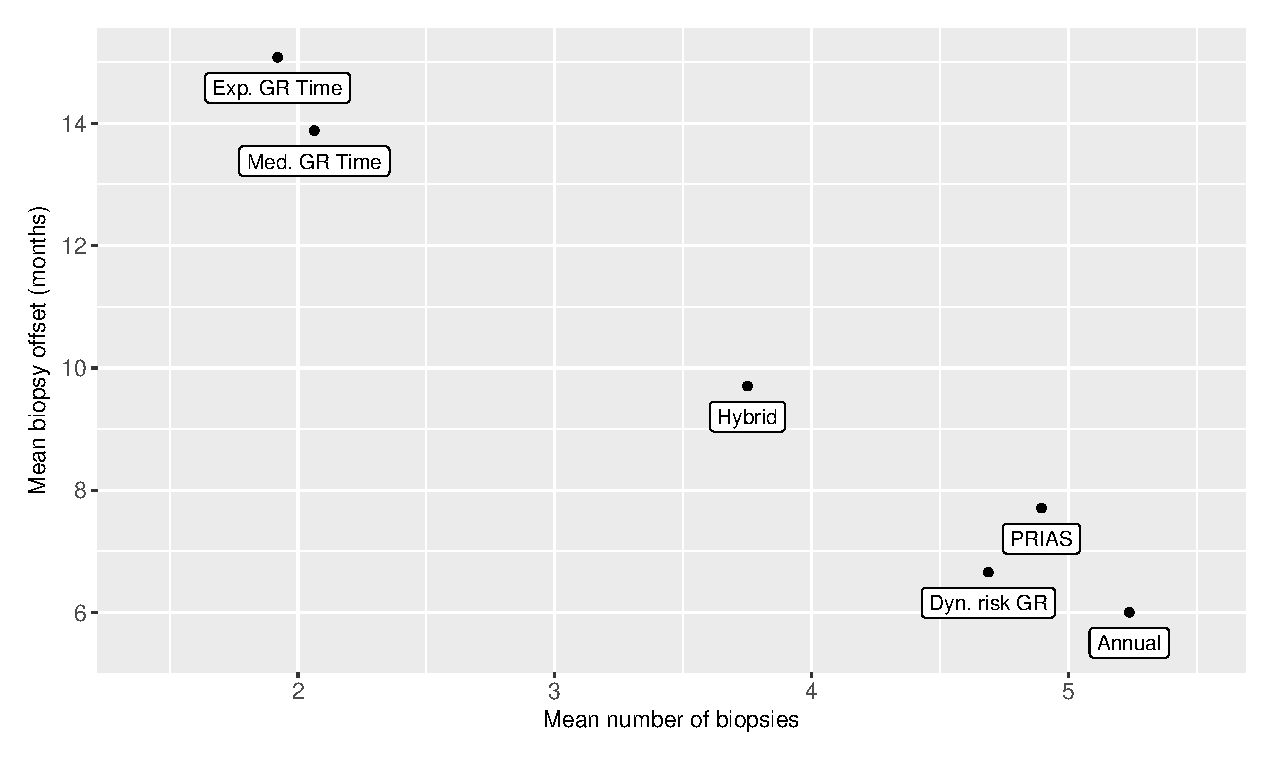
\includegraphics[width=\columnwidth]{images/sim_study/meanNbVsOffset_all.eps}}
\caption{Estimated mean number of biopsies and mean offset (months) for the 6 schedules, using all simulated patients.}
\label{fig : meanNbVsOffset}
\end{figure}

%124781 = 41484 + 41423 + 41874
\begin{table}
\caption{Estimated mean and standard deviation of the number of biopsies and offset (months).}
\label{table : sim_study_pooled_estimates}
\begin{tabular}{lrrrr}
\Hline
\multicolumn{5}{c}{a) All subgroups}\\
\hline
Schedule          & $E(N^S_j)$ & $E(O^S_j)$ & ${\mbox{SD}(N^S_j)}$ & ${\mbox{SD}(O^S_j)}$ \\
\hline
Annual         & 5.24            & 6.01                & 2.53          & 3.46              \\
PRIAS          & 4.90            & 7.71                & 2.36          & 6.31\\
Dyn. risk GR       & 4.69            & 6.66                & 2.19           & 4.38              \\
Hybrid       & 3.75            & 9.70                & 1.71          & 7.25              \\
Med. GR time & 2.06            & 13.88               & 1.41          & 11.80              \\
Exp. GR time & 1.92            & 15.08               & 1.19          & 12.11             \\
\hline
\multicolumn{5}{c}{b) Subgroup $G_1$}\\
\hline
Schedule        & $E(N^S_j)$ & $E(O^S_j)$ & ${\mbox{SD}(N^S_j)}$ & ${\mbox{SD}(O^S_j)}$ \\
\hline
Annual         & 4.32            & 6.02                & 3.13          & 3.44              \\
PRIAS          & 4.07            & 7.44                & 2.88          & 6.11    \\
Dyn. risk GR       & 3.85            & 6.75                & 2.69          & 4.44              \\
Hybrid       & 3.25            & 10.25               & 2.16          & 8.07              \\
Med. GR time & 1.84            & 20.66               & 1.76          & 14.62             \\
Exp. GR time & 1.72            & 21.65               & 1.47          & 14.75             \\
\hline      
\multicolumn{5}{c}{c) Subgroup $G_2$}\\
\hline
Schedule        & $E(N^S_j)$ & $E(O^S_j)$ & ${\mbox{SD}(N^S_j)}$ & ${\mbox{SD}(O^S_j)}$ \\
\hline
Annual         & 5.18            & 5.98                & 2.13          & 3.47              \\
PRIAS          & 4.85            & 7.70                & 2.00          & 6.29        \\
Dyn. risk GR       & 4.63            & 6.66                & 1.82          & 4.37              \\
Hybrid       & 3.68            & 10.32                & 1.37          & 7.45              \\
Med. GR time & 1.89             & 12.33               & 1.16          & 9.44              \\
Exp. GR time & 1.77            & 13.54               & 0.98          & 9.83              \\
\hline      
\multicolumn{5}{c}{d) Subgroup $G_3$}\\
\hline
Schedule        & $E(N^S_j)$ & $E(O^S_j)$ & ${\mbox{SD}(N^S_j)}$ & ${\mbox{SD}(O^S_j)}$ \\
\hline
Annual         & 6.20             & 6.02                & 1.76          & 3.46              \\
PRIAS          & 5.76             & 7.98                & 1.71         & 6.51        \\
Dyn. risk GR       & 5.58            & 6.58                & 1.56          & 4.33              \\
Hybrid       & 4.32            & 8.55                & 1.26          & 5.91              \\
Med. GR time & 2.45            & 8.70                & 1.15          & 6.32              \\
Exp. GR time & 2.27            & 10.09               & 0.99          & 7.47              \\
\hline     
\end{tabular}
\end{table}

The PRIAS schedule conducts only 0.3 biopsies less than the annual schedule, but with a higher variance of offset, it does not guarantee early detection for everyone. If we compare the PRIAS schedule with dynamic risk of GR based schedule, we can see that the latter performs slightly better than PRIAS schedule in all four criteria. The hybrid approach combines the benefits of methods with low $E(N^S_j)$ and $\mbox{SD}(N^S_j)$, and methods with low $E(O^S_j)$ and $\mbox{SD}(O^S_j)$. It conducts 1.5 biopsies less than the annual schedule on average and with a $E(O^S_j)$ of 9.7 months it detects GR within an year since its occurrence. Moreover, it has both $\mbox{SD}(N^S_j)$ and $\mbox{SD}(O^S_j)$ comparable to PRIAS.

The performance of each schedule differs for the three subgroups $G_1, G_2$ and $G_3$. The annual schedule remains the most consistent across subgroups in terms of the offset, but it conducts 2 extra biopsies for subgroup $G_3$ (slowly progressing PCa) than $G_1$ (faster progressing PCa). The performance of schedule based on expected time of GR is the most consistent in terms of number of biopsies but it detects GR an year later on average in subgroup $G_1$ than $G_3$. For the dynamic risk of GR based schedule and the hybrid schedule the dynamics are similar to that of the annual schedule. Unlike the latter two schedules, the PRIAS schedule not only conducts more biopsies in $G_3$ than $G_1$ but also detects GR later in $G_3$ than $G_1$.

\begin{figure}[!htb]
\centerline{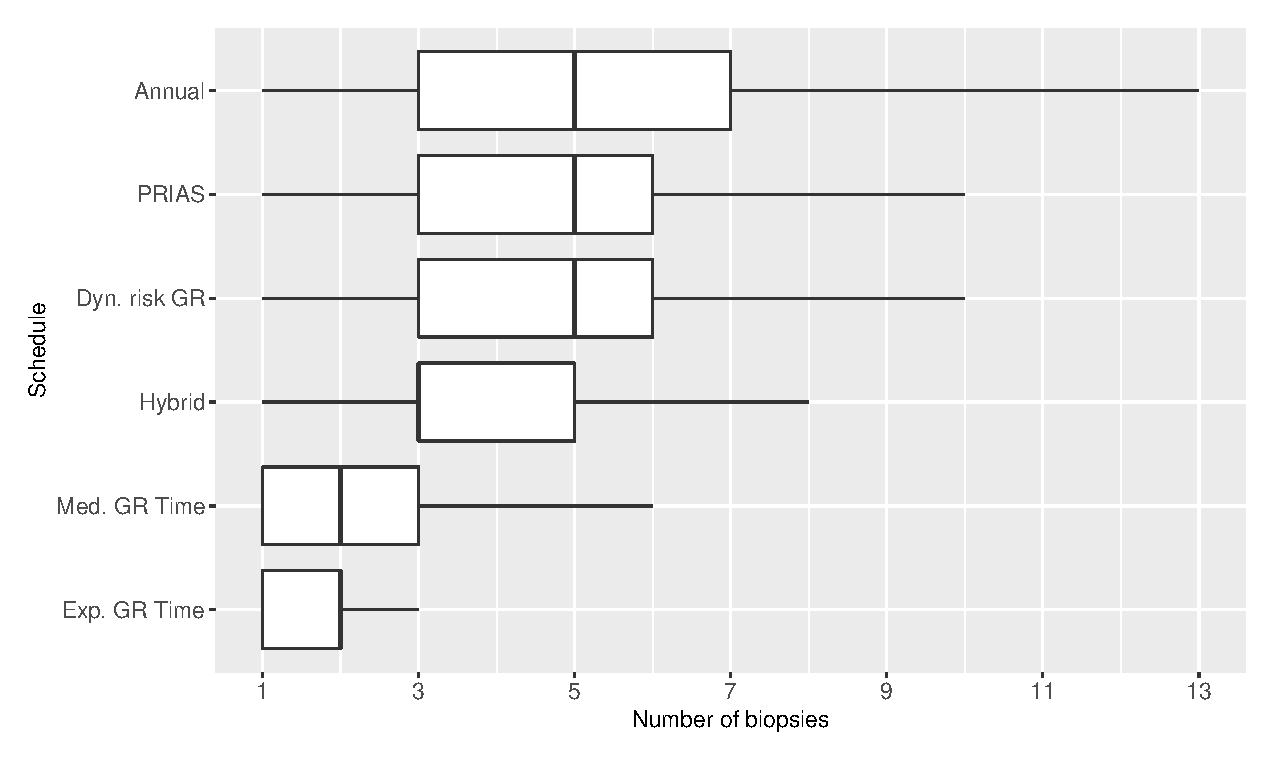
\includegraphics[width=\columnwidth]{images/sim_study/nbBoxPlot_all.eps}}
\caption{Boxplot showing variation in number of biopsies conducted by different methods, using all simulated patients.}
\label{fig : nbBoxPlot_all}
\end{figure}

\begin{figure}[!htb]
\centerline{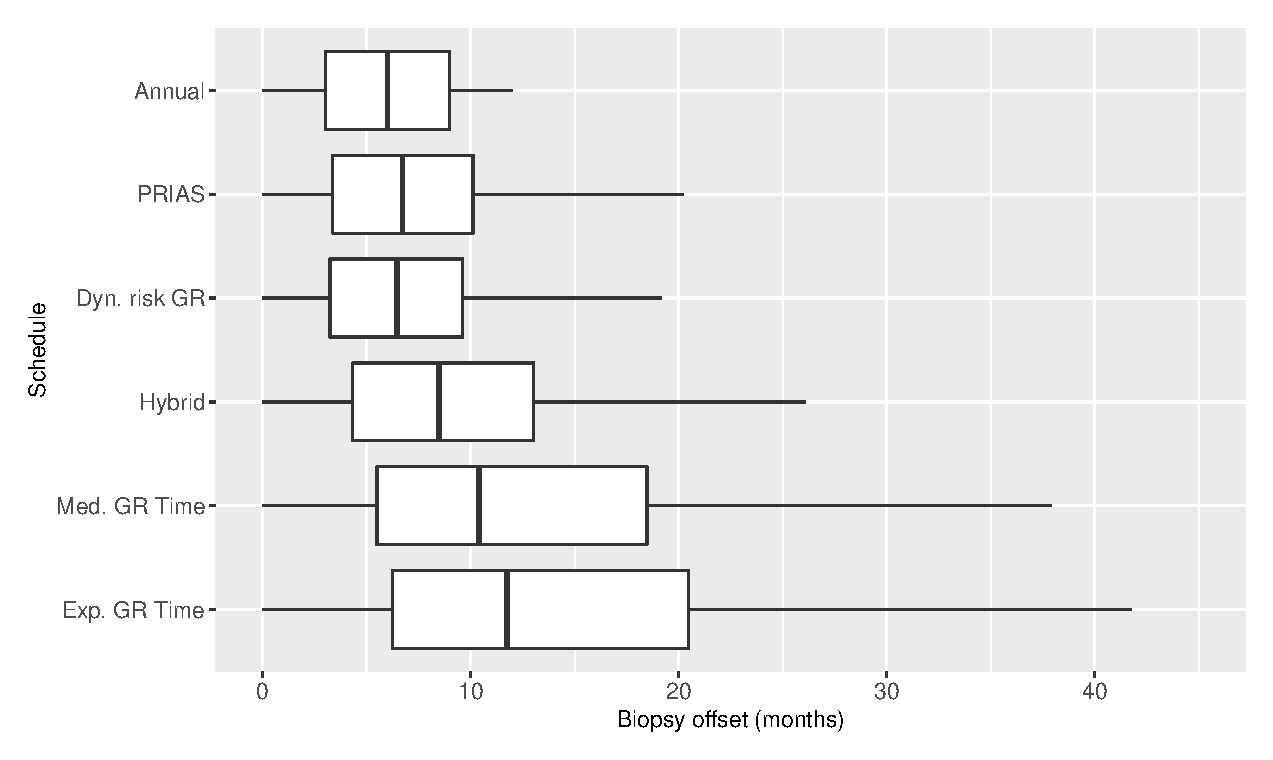
\includegraphics[width=\columnwidth]{images/sim_study/offsetBoxPlot_all.eps}}
\caption{Boxplot showing variation in biopsy offset (months) for different methods, using all simulated patients.}
\label{fig : offsetBoxPlot_all}
\end{figure}

The choice of a suitable schedule using (\ref{eq : loss_func_sim_study_generic}) depends on the chosen criteria for evaluation of schedules. For example, the schedule based on dynamic risk of GR is suitable if on average the least number of biopsies are to be conducted to detect GR, while simultaneously making sure that at least 90\% of the patients have an average offset less than one year (Figure \ref{fig : nbBoxPlot_all} and \ref{fig : offsetBoxPlot_all}). The schedule based on expected time of GR is suitable if on average the least number of biopsies are to be conducted to detect GR, while simultaneously making sure that at least 90\% of the patients have an average offset less than three years. If a stricter cutoff is required on offset the hybrid approach may be suitable, since it conducts only 3.8 biopsies on average while guaranteeing an offset of two years for 95\% of the patients and three years for 99.9\% of the patients. Besides if further cutoffs are required on variance of number of biopsies or offset they are not too high either for the hybrid approach.